\textbf{Data and manual data handling} \newline
Data used in this study were collected beforehand from an on-going clinical trial (FOXH) which is conducted in collaboration with Danish and Australian universities. The data consists of pain maps which were drawn by individuals with PFPS through the use of an application, Navigate Pain, in a clinical setting. The pain maps are both from individuals with uni- and bilateral PFP, an example of these are shown in fig. \ref{fig:twoPainmaps}.

\begin{figure}[H]
\centering
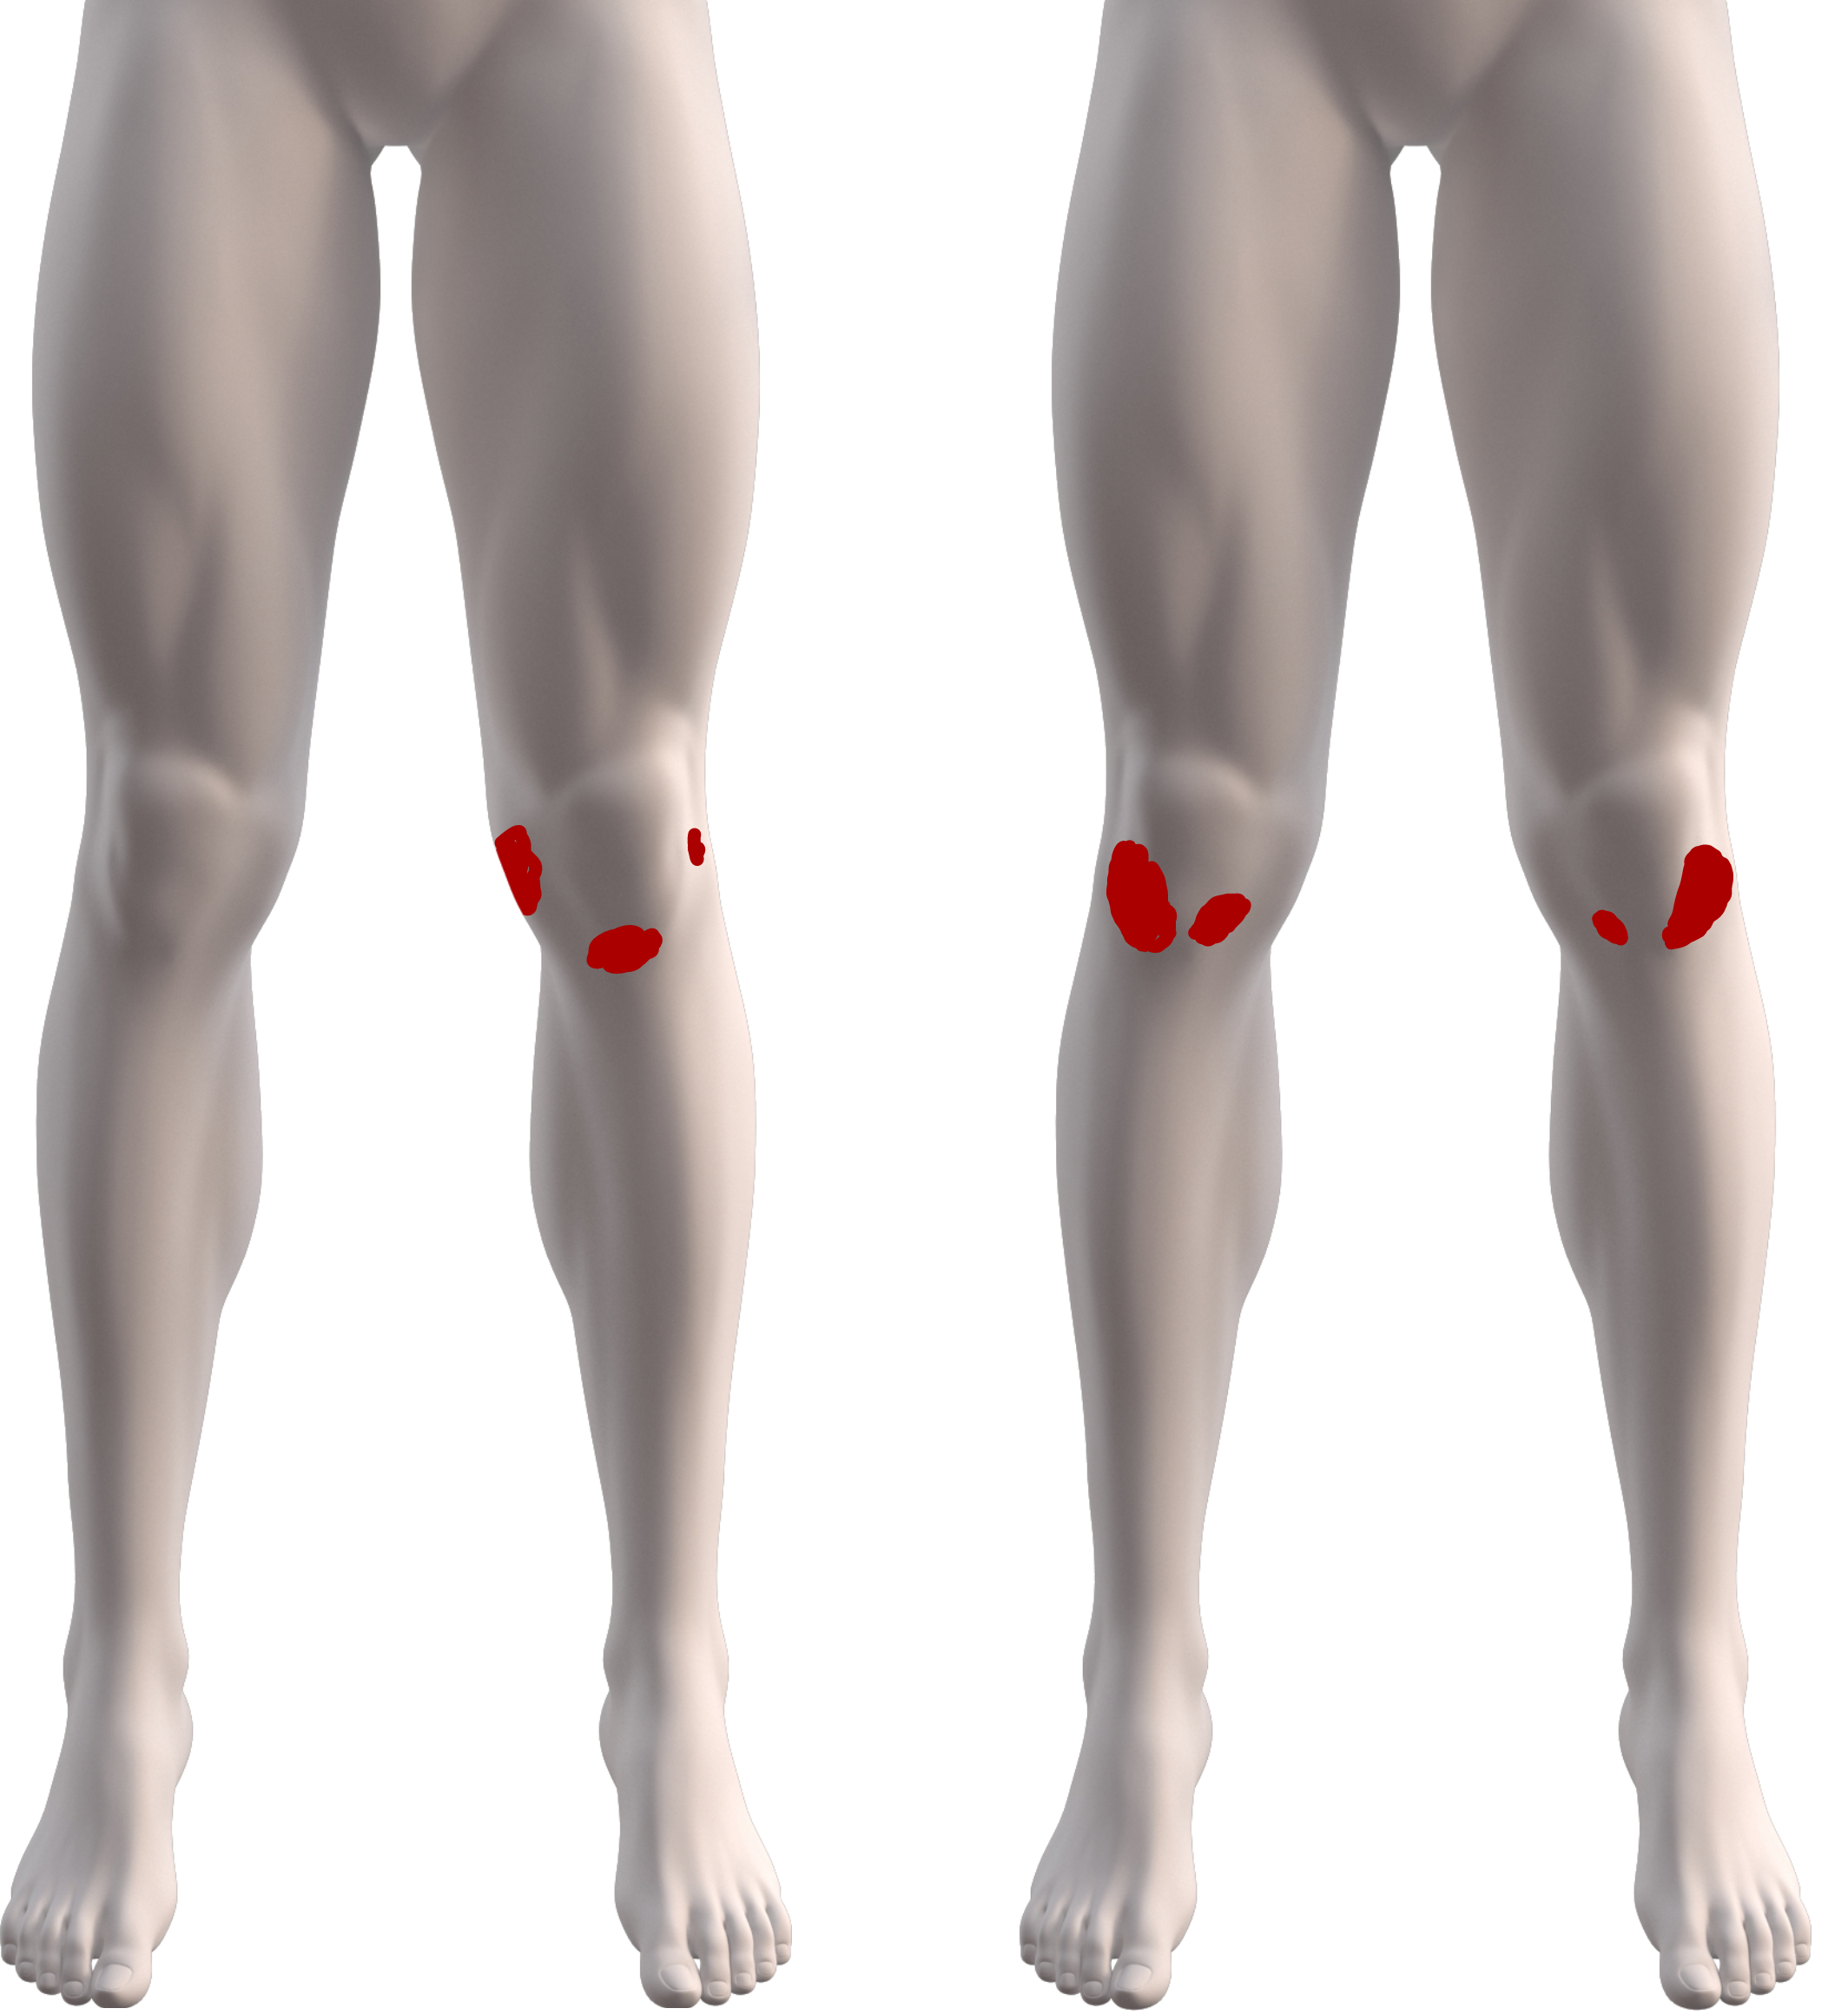
\includegraphics[width=0.4\textwidth]{Figures/twoPainmaps}
\caption{Pain maps from individuals with uni- and bilateral PFP. The red markings indicate the area of pain perceived by the individuals.}
\label{fig:twoPainmaps}
\end{figure}

\noindent
In addition to the pain maps related information regarding the individuals was available.
Before using the data in the deep learning models, a manual data handling was necessary to match the given pain maps and associated ID on the individuals, which resulted in 217 available pain maps. Furthermore, specific information like gender, symptom duration and pain intensity were collected from the appurtenant information. The number of pain maps with associated gender and symptom duration, was 205. Additionally, there were 197 pain maps with associated gender and pain intensity.\\

\noindent
\textbf{Software application: Navigate Pain} \newline
Navigate Pain is a software application that is used to visualise the location, morphology and spatial distribution of pain from individuals to healthcare personnel. The application permits individuals to draw their pain with different colors and line thickness onto a body outline. Navigate Pain android was developed at Aalborg University and a commercial web application is available at Aglance Solutions (Denmark).\citep{Solutions2015}\\

\noindent
\textbf{Knee regions} \newline
\noindent
To define the location of the PFP the knees are divided into 20 regions, which are inspired by Photographic Knee Pain Map (PKPM). The divisions are designed to categorise location of knee pain for diagnostic and research purposes. PKPM represent both knees that makes it possible to identify unilateral and bilateral pain.\citep{Elson2010} The knee regions are illustrated in fig. \ref{fig:atlas}.

\begin{figure} [H] 
\centering
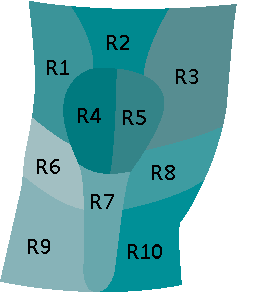
\includegraphics[width=0.38\textwidth]{Figures/atlas}
\caption{The regions of the left (L1-L10) and right (R1-R10) knees, where each knee is split into ten regions.}
\label{fig:atlas}
\end{figure}

\noindent
The regions are based on the anatomical structures according to the areas where individuals often indicate pain.
There are ten regions on each knee, where region 1 and 3 represent the superior lateral and superior medial areas for patella. Region 2 refers to quadriceps tendon. The patella is divided into lateral and medial regions, which are region 4 and 5. Region 6 and 8 are lateral and medial joint line areas. Patella tendor is region 7 and the two last regions, 9 and 10, are tibia lateral and medial.\citep{Elson2010}

\noindent
\textbf{Data representations} \newline
\noindent
To investigate whether morphology and location of pain have an influence on the outputs, symptom duration and pain intensity, the pain maps are encoded in multiple data representations. The pain maps were processed in MatLab, where the images were resized, since they were collected at different resolutions (screen sizes) and cropped to sort out unnecessary data like the areas inferior and superior to the knee.  Each data representation is reflected in a matrix consisting of the pain maps, gender and the output, symptom duration and pain intensity. Since the original pain maps reflecting the morphology of the pain, thus the morphology-representation does not require further manipulation. \newline
\noindent
To investigate whether the location alone have a correlation to the outputs, a simplified representation of the pain maps are created. The location of the pain is then reflected by the use of the defined knee regions (fig. \ref{fig:atlas}), where each region represent a value of 0 (not active) or 1 (active) in a vector.  The values were defined by using a threshold to determine whether a region was considered active in relation the amount of pain. A threshold was required to increase the confidence of an active pain region by avoiding minimal contributions e.g. small pain areas in the associated regions. Simultaneously the threshold should not be too large so that pain areas was excluded. The threshold was decided based on an analysis on five random pain maps, where threshold values of 0, 5, 10 and 15\% was compared. The threshold represent which minimal percentage of pain should be present in a specific region before it is considered active. Based on the analysis a 5\% threshold was chosen. \newline
\noindent
Lastly, a data representation which reflects a combination of morphology and location of the pain, is prepared to explore if the interaction of morphology and location of pain would give a better classification according to the outputs.


- Simple regression
- Deep learning + modeller